%&pdflatex
\documentclass[smallextended, referee]{svjour3} % svjour3: smallextended, referee
\usepackage[english]{babel}
\usepackage[T1]{fontenc}
\usepackage{graphicx}
\usepackage{amssymb, amsmath}
\usepackage{endfloat}
\usepackage{cite}
\usepackage{fixltx2e}
\usepackage{fullpage}

\newcommand{\Kn}{\mathrm{Kn}}
\newcommand{\dd}{\:\mathrm{d}}
\newcommand{\pder}[2][]{\frac{\partial#1}{\partial#2}}
\newcommand{\pderder}[2][]{\frac{\partial^2 #1}{\partial #2^2}}
\newcommand{\Pder}[2][]{\partial#1/\partial#2}

\journalname{Theoretical and Computational Fluid Dynamics}

\begin{document}

\title{
	Computer simulation of slightly rarefied gas flows driven by significant temperature variations and their continuum limit
}

\author{O.A.~Rogozin}
\institute{O.A.~Rogozin \at
	Moscow Institute of Physics and Technology,
	9 Institutskiy pereulok, g. Dolgoprudny,
	Moskovskaya obl., Russian Federation\\
	\email{o.a.rogozin@gmail.com}  
}

\maketitle

\begin{abstract}
	Classical fluid dynamics describes a behavior of gas in terms of the
	Navier--Stokes equations. However, a rigorous asymptotic analysis of
	the Boltzmann equation for small Knudsen numbers restricts the scope
	of its application and in a general case leads to more complicated
	sets of differential equations. Present paper deals with such one
	that is valid for significant temperature variations and finite
	Reynolds numbers. A special-purpose solver on the open-source CFD
	platform OpenFOAM\textregistered{} is proposed for computer
	simulation of a slightly rarefied gas in an arbitrary geometry. Some
	temperature driven flows are considered as examples.
	\keywords{
		OpenFOAM \and
		Boltzmann equation \and
		Navier--Stokes equations \and
		thermal creep flow \and
		nonlinear thermal-stress flow \and
		ghost effect
	}
	\PACS{47.45.-n,47.11.Df}
\end{abstract}

\section{Introduction}

%%% Current state of affairs
The Navier--Stokes equations is widely used equations for modeling of a gas with the vanishing mean free path.
Slightly rarefied gas effects, which is widely thought to take place only in the thin Knudsen layer,
can be taken into account using the slip conditions on the boundary~\cite{SharipovCoefficients}.
In some situations, however, the Navier--Stokes set fails to describe the correct temperature field
even in the continuum limit~\cite{Kogan1976, GhostEffect}.
When the Reynolds number is finite and the temperature variations are large:
\[ \mathrm{Re} = O(1), \quad \frac1T\left|\pder[T]{x_i}\right| = O(1), \]
higher-order terms of gas rarefaction begin to play a significant role in the gas behavior.
In this case, the asymptotic analysis of the Boltzmann equation arrives on the scene and
yields the appropriate equations on the macroscopic variables, together with
their associated boundary conditions~\cite{Sone2002, Sone2007}.

%%% Existing solutions
This new set of equations has the similar structure to the Navier--Stokes one,
so similar numerical methods can be utilized too.
The pioneering solutions are based on the finite difference methods~\cite{GhostEffect, Kogan1976}.
The finite volume method are applied in some recent works~\cite{Laneryd2006, Laneryd2007}.

%%% Limitations
Nowadays, many CFD platforms provide comprehensive
capabilities for numerical simulation of the Navier--Stokes equations,
but the considered fluid-dynamic-type set of equations remains in the shadow.
The present paper aims to improve this situation and
draw more attention to such CFD scope extensions.

%%% Why OpenFOAM?
One of the modern and promising CFD platforms, OpenFOAM\textregistered{}
has been selected as a basis for numerical algorithms developing.
OpenFOAM\textregistered{} is an object-oriented C++ library of classes and routines for parallel computation,
providing a set of high-level tools for writing advanced CFD code~\cite{OpenFOAM1998}.
It has a wide set of basic features, similar to any commercial one~\cite{OpenFOAM2010},
and is a robust and reliable software widely used in the industry~\cite{BoilingFlows2009,
TurbulentCombustion2011, CoastalEngineering2013, BiomassPyrolysis2013}.
As for rarefied gas, OpenFOAM\textregistered{} has a standard solver for DSMC, that
can be extended for hybrid simulations~\cite{HybridSolver2012}.
Finally, the most important advantage of OpenFOAM\textregistered{} is its open-source code,
so it is easy to add any modification to any part of the implementation.
OpenFOAM\textregistered{} is also well documented and has a large and active community of users.

\section{Basic equations}

Gases are described by the conservation laws of mass, momentum and energy:
\begin{gather}
	\pder[\rho]{t} + \pder{x_i}(\rho v_i) = 0, \label{eq:mass}\\
	\pder{t}(\rho v_i) + \pder{x_j}(\rho v_i v_j + p_{ij}) = \rho F_i, \label{eq:momentum}\\
	\pder{t}\left[\rho\left(e+\frac{v_i^2}2\right)\right] +
		\pder{x_j}\left[\rho v_j\left(e+\frac{v_i^2}2\right)+v_i p_{ij}+q_j\right] = \rho v_j F_j. \label{eq:energy}
\end{gather}
Macroscopic variables have the following notation: the density \(\rho\), the flow velocity \(v_i\), the stress tensor \(p_{ij}\),
the specific internal energy \(e\), and the heat-flow vector \(q_i\). Finally, \(F_i\) denotes the external force.
For an ideal monatomic gas, the internal energy \(e\) depends only on the temperature \(T\):
\[ e = \frac32RT, \]
where \(R = k_B / m\) is the specific gas constant. The pressure is taken from the equation of state:
\[ p = \rho RT. \]

The conservation equations are closed to the Navier--Stokes set by means of the Newton and Fourier laws
for the stress tensor \(p_{ij}\) and the heat-flow vector \(q_i\), respectively:
\begin{gather}
	p_{ij} = p\delta_{ij} - \mu\left(\pder[v_i]{x_j}+\pder[v_j]{x_i}-\frac23\pder[v_k]{x_k}\delta_{ij}\right) -
		\mu_B\pder[v_k]{x_k}\delta_{ij}, \label{eq:stress_tensor}\\
	q_i = -\lambda\pder[T]{x_i}. \label{eq:heat_flow}
\end{gather}
Transport coefficients are given above:
the viscosity \(\mu\), the second viscosity \(\mu_B\), and the thermal conductivity \(\lambda\).

A Knudsen number \(\Kn\) is determined by the ratio of the mean free path
\begin{equation}\label{eq:ell}
	\ell = \frac{m}{\sqrt2\pi d_m^2 \rho}.
\end{equation}
to the characteristic dimension of the problem \(L\):
\begin{equation}\label{eq:Knudsen}
	\Kn = \frac{\ell}L.
\end{equation}
It is convenient to deal with a modified Knudsen number:
\begin{equation}
	k = \frac{\sqrt\pi}2\Kn.
\end{equation}
For a hard-sphere gas, the radius of the intermolecular force influence \(d_m\)
coincides with the diameter of a molecule.

Further variables are assumed dimensionless with corresponding reference units:
the length \(L\), the pressure \(p^{(0)}\), the temperature \(T^{(0)}\),
the velocity \((2RT^{(0)})^{1/2}\) and the heat-flow vector \(p^{(0)}(2RT^{(0)})^{1/2}\).

The viscosity \(\mu\) and the thermal conductivity \(\lambda\) of an ideal gas
are proportional to the mean free path \(\ell\), and thus to the Knudsen number:
\begin{equation}
	\mu = O(k), \quad \lambda = O(k).
\end{equation}
For \(k\to0\) we obtain the Euler set of equations:
\begin{equation}
	p_{ij} = p\delta_{ij}, \quad q_i = 0.
\end{equation}

However, the Euler set failed to determine the temperature field.
Classical heat-conduction equation is derived from~\eqref{eq:energy} and~\eqref{eq:heat_flow}
in the absence of gas motion \(v_i = 0\):
\begin{equation}\label{eq:heat_equation}
	\pder{x_i}\left(\sqrt{T}\pder[T]{x_i}\right) = 0.
\end{equation}
Here, it takes into account that the thermal conductivity of a hard-sphere gas is proportional to \(\sqrt{T}\).

\section{Asymptotic analysis of the Boltzmann equation}

A detailed mathematical derivation of the following results can be found in~\cite{Sone2002, Sone2007}.

\subsection{Fluid-dynamic-type equations}

The analysis presented below is based on the conventional Hilbert expansion
of the distribution function \(f\) and macroscopic variables \(h\)~\cite{Hilbert1912}:
\[ f = f_0 + f_1k + f_2k^2 + \cdots, \quad h = h_0 + h_1k + h_2k^2 + \cdots \]
with the additional condition
\begin{equation}\label{eq:Mach_constraint}
	u_{i0} = 0.
\end{equation}
meaning that the Mach number is of the same order as the Knudsen number.
Pressures \(p_0\) and \(p_1\) are constant due to degenerated Euler equation
\(\Pder[p_0]{x_i} = 0 \) and \(\Pder[p_1]{x_i} = 0 \).

The following set of equations is resulted for variables \(T_0\), \(u_{i1} = p_0v_{i1}\), \(p_2^\dag\):
\begin{align}
	\pder{x_i}\left(\frac{u_{i1}}{T_0}\right) &= 0, \label{eq:asymptotic1} \\
	\pder{x_j}\left(\frac{u_{i1}u_{j1}}{T_0}\right)
		&-\frac{\gamma_1}2\pder{x_j}\left[\sqrt{T_0}\left(
			\pder[u_{i1}]{x_j}+\pder[u_{j1}]{x_i}-\frac23\pder[u_{k1}]{x_k}\delta_{ij}\right
		)\right] \notag\\
		&- \frac{\gamma_7}{T_0}\pder[T_0]{x_i}\pder[T_0]{x_j}\left(\frac{u_{j1}}{\gamma_2\sqrt{T_0}} - \frac{1}4\pder[T_0]{x_j}\right) \notag\\
		&= -\frac1{2p_0}\pder[p_2^\dag]{x_i}, \label{eq:asymptotic2} \\
	\pder[u_{i1}]{x_i} &= \frac{\gamma_2}2\pder{x_i}\left(\sqrt{T_0}\pder[T_0]{x_i}\right), \label{eq:asymptotic3}
\end{align}
where
\[ 
	p_2^\dag = p_2 + 
		\frac{2\gamma_3}{3p_0}\pder{x_k}\left(T_0\pder[T_0]{x_k}\right) -
		\frac{\gamma_7}{6p_0}\left(\pder[T_0]{x_k}\right)^2.
\]
The set of equations \eqref{eq:asymptotic1}--\eqref{eq:asymptotic3} has a fluid-dynamic nature
and is comparable to the Navier--Stokes equations for a compressible gas (\(\rho_0 = p_0/T_0\)).
The formal difference consists in the additional thermal stress terms.
Furthermore, \(p_2^\dag\) is not included in the equation of state,
so it is determined up to a constant factor.
Term \(\partial{p_2 ^ \dag} / \partial{x_i}\) participates in the system as the pressure
in the Navier--Stokes set for incompressible gas.
This fact specifies the corresponding numerical methods for solving \eqref{eq:asymptotic1}--\eqref{eq:asymptotic3}.

For a hard-sphere gas, dimensionless transport coefficients are equal
\begin{alignat*}{2}
	\gamma_1 &= 1.270042427, &\quad \gamma_2 &= 1.922284066, \\
	\gamma_3 &= 1.947906335, &\quad \gamma_7 &= 1.758705.
\end{alignat*}
The first two ones are related to the viscosity \(\mu\) and
the thermal conductivity \(\lambda\) for a hard-sphere gas:
\begin{equation}
	\mu = \gamma_1\sqrt{T_0} \frac{p^{(0)}L}{\sqrt{2RT^{(0)}}} k, \quad
	\lambda = \frac{5\gamma_2}{2}\sqrt{T_0} \frac{p^{(0)}RL}{\sqrt{2RT^{(0)}}} k,
\end{equation}	
and \(\gamma_7\) is related to the \emph{nonlinear thermal-stress flow}.

\subsection{Boundary conditions}

The fluid-dynamic boundary conditions based on the diffuse-reflection boundary conditions
for Boltzmann equation look as follows:
\begin{gather}
	T_0 = T_B, \label{eq:bound:T} \\
	\left\{
	\begin{aligned}
		& \frac{(u_{j1}-u_{Bj1})}{\sqrt{T_B}}(\delta_{ij}-n_in_j) = 
			-K_1\pder[T_B]{x_j}(\delta_{ij}-n_in_j), \\
		& u_{j1}n_j = 0.
	\end{aligned}
	\right. \label{eq:bound:v}
\end{gather}
Here, \(n_i\) is the unit normal vector to the boundary pointing into the gas,
\(u_{Bj1}\), \(T_B\) are the velocity and the temperature of the boundary.
\(K_1\) is the dimensionless slip coefficient for the \emph{thermal creep flow}. For a hard-sphere gas,
\[ K_1 = -0.6463. \]

The solution of the boundary-value problem cannot be expressed only with the fluid-dynamic-type
solution due to the sharp variation in the distribution function near the boundary.
Therefore, it is necessary to introduce the so-called Knudsen-layer correction:
\begin{equation}
	f = f_{FD} + f_K, \quad h = h_{FD} + h_K.
\end{equation}
The fluid-dynamic part \(f_{FD}\) is the solution presented above,
and \(f_K\) decays exponentially with the distance to the boundary \(f_K = O\left(e^{-\eta}\right)\).
The relation \( x_i = k\eta n_i(s_1,s_2) + x_{Bi}(s_1, s_2) \) gives a coordinate transformation
from \((x_1,x_2,x_3)\) to \((\eta,s_1,s_2)\).

Due to the infinitesimal Mach number (\ref{eq:Mach_constraint}) \(f_K\) is expanded
in a power series of \(k\), starting from the first order:
\[ f_K = f_{K1} k + f_{K2} k ^ 2 + \cdots \]
The Knudsen layer introduces a correction to \(u_{i1}\) for a hard-sphere gas:
\begin{equation}
	\left\{
	\begin{aligned}
		& \frac{u_{jK1}}{\sqrt{T_B}}(\delta_{ij}-n_in_j) =
			-\frac12\pder[T_B]{x_j} Y_1\left(\frac\eta{T_B}\right) (\delta_{ij}-n_in_j), \\
		& u_{jK1}n_j = 0.
	\end{aligned}
	\right. \label{eq:bound:v_K}
\end{equation}
The function \(Y_1(\eta)\) is tabulated, for example, in~\cite{Sone2002, Sone2007} and is shown in Fig.~\ref{fig:Y1}.

\begin{figure}[ht]
	\centering
	\begin{minipage}{.48\textwidth}
		\centering
		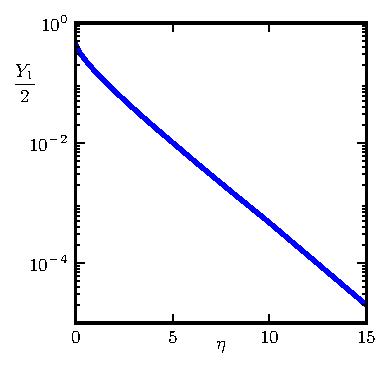
\includegraphics{Fig1}
		\caption{The function of the Knudsen layer \(Y_1(\eta)/2\) for a hard-sphere gas.}
		\label{fig:Y1}
	\end{minipage}
	\quad
	\begin{minipage}{.48\textwidth}
		\centering
		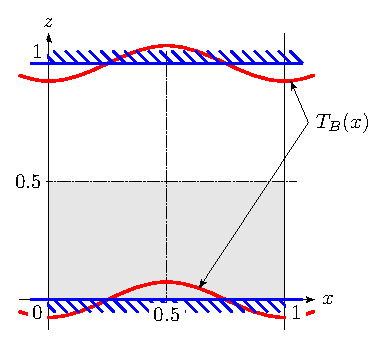
\includegraphics{Fig2}
		\vspace{13pt}
		\caption{Geometry of the problem: the gas is placed between two parallel plates
			with the periodical temperature distribution \(T_B\).}
		\label{fig:geometry}
	\end{minipage}
\end{figure}

\subsection{Some remarks on the continuum limit}

As one can see from~\eqref{eq:asymptotic3}, gas is not always described correctly
by the heat-conduction equation~\eqref{eq:heat_equation}.
Equation~\eqref{eq:asymptotic3} converges to~\eqref{eq:heat_equation} only if \(u_{i1} = 0\).
This condition is not satisfied in three different cases:
\begin{enumerate}
	\item The boundary is moving with the velocity of the order of k: \(u_{B1i} \neq 0 \).
	\item The boundary temperature is not uniform (thermal creep flow): \(\Pder[T_B]{x_i} \neq 0 \).
	\item The isothermal surfaces are not parallel (nonlinear thermal-stress flow):
		\begin{equation}\label{eq:equilibrium}
			e_{ijk}\pder[T_0]{x_j}\pder{x_k}\left(\pder[T_0]{x_l}\right)^2 \neq 0.
		\end{equation}
\end{enumerate}

The first two cases are directly determined by the boundary conditions,
and the third one has only an implicit impact from them.

The set of equations~\eqref{eq:asymptotic1}--\eqref{eq:asymptotic3} revealed the following interesting fact.
In the continuum limit, the gas flows vanish, proportional to the Knudsen number.
However, the infinitesimally weak flows have a finite impact on the temperature field.
This asymptotic behavior is called the \emph{ghost effect}~\cite{GhostEffect, Sone2002, Sone2007}.

\section{Numerical simulation and discussions}

\begin{figure}[ht]
	\centering
	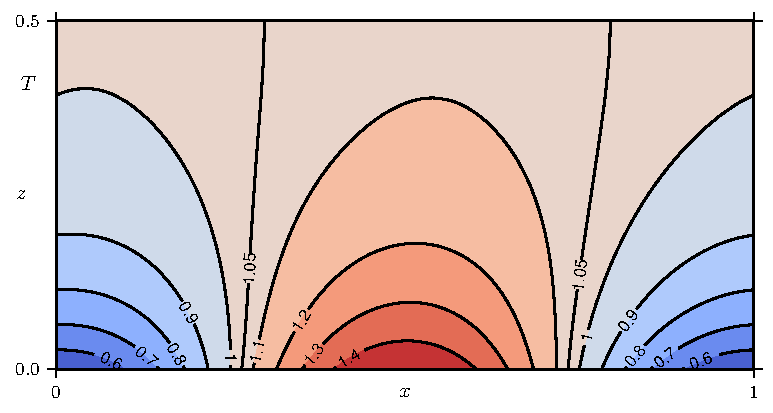
\includegraphics{Fig3}
	\caption{The temperature field \(T\), obtained from the asymptotic theory in the continuum limit:
		isothermal lines are placed above the contour lines.}
	\label{fig:moving:T_asym}
\end{figure}

\begin{figure}[ht]
	\centering
	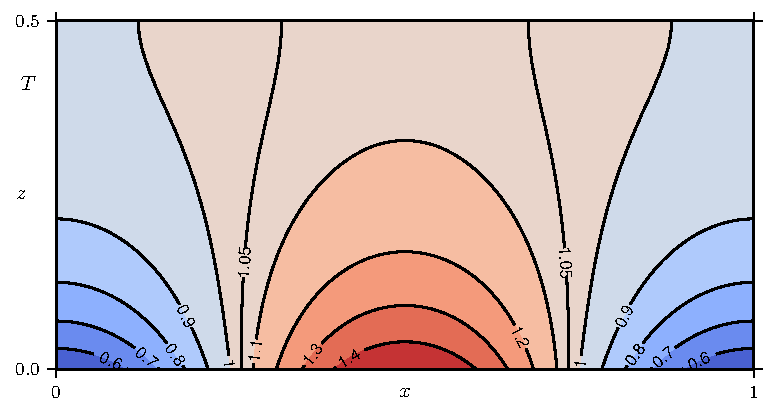
\includegraphics{Fig4}
	\caption{Temperature field \(T\), obtained from the heat-conduction equation:
		isothermal lines are placed above the contour lines.}
	\label{fig:moving:T_heat}
\end{figure}

Present results are obtained with the special solver of the system~\eqref{eq:asymptotic1}--\eqref{eq:asymptotic3}.
It has been developed within the open-source CFD toolbox OpenFOAM\textregistered{}~\cite{OpenFOAM1998},
based on the finite-volume approach for evaluating partial derivatives.
The continuity equation~\eqref{eq:asymptotic1}, along with the momentum equation~\eqref{eq:asymptotic2},
is solved with the commonly used implicit conservative SIMPLE algorithm~\cite{SIMPLE}.
A detailed description of this scheme for gas mixtures can be found in~\cite{Laneryd2007}.

Unstructured spacial grids are generated with the open-source package GMSH~\cite{GMSH}.
They are nonuniform and condensed in areas with large gradients of macroscopic variables.
From \(10^3\) to \(10^6\) cells are used to achieve the residual of the solution
that is not greater than \(10^{-6}\) for all considered problems.

OpenFOAM\textregistered{} uses Kitware's ParaView\textregistered{} as a primary visualization system of results,
but for present paper another open-source tool Matplotlib was chosen to create color vector illustrations.

All transport coefficients are taken in compliance with the hard-sphere model.
Complete diffuse reflection is assumed from a solid boundary.

\subsection{Gas between two parallel plates}

Consider a plane periodic geometry shown in Fig.~\ref{fig:geometry}.
The gas is placed between two infinite parallel plates
that have a sinusoidal distribution of the temperature
\begin{equation}
	T_B = 1-\alpha\cos(2\pi x).
\end{equation}
Lower plate moves relative to the top with the velocity
\begin{equation}
	u_{Bi} = (\beta\Kn,0,0).
\end{equation}

The first example of simulation is for
\[ \alpha=1/2, \quad \beta = 1. \]

Due to the problem symmetry, computational domain represents a rectangle \(0<x<1, 0<z<1/2\)
(a gray background in Fig.~\ref{fig:geometry}).

\begin{figure}
	\centering
	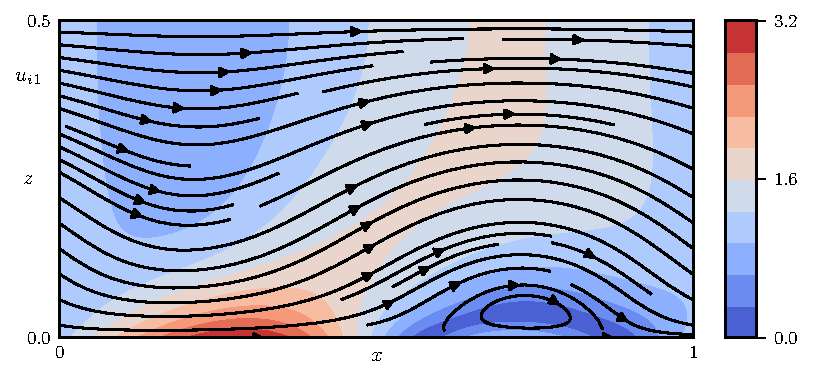
\includegraphics{Fig5}
	\caption{The fluid-dynamic part of the velocity field \(u_{FDi1}\):
		curves with arrows indicate the direction, contour lines show the magnitude.}
	\label{fig:moving:fluid}
\end{figure}

\begin{figure}
	\centering
	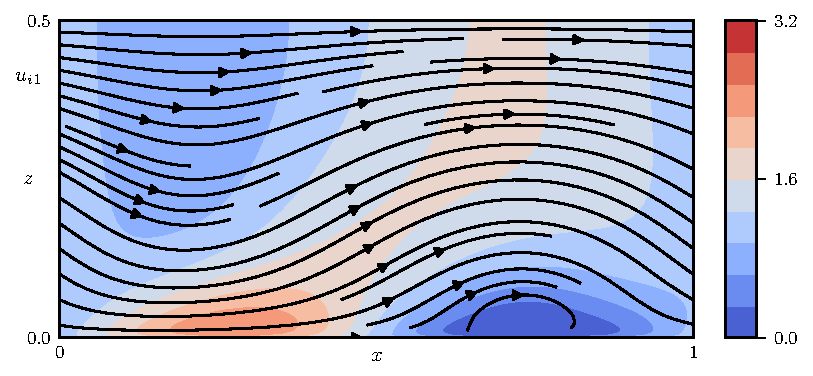
\includegraphics{Fig6}
	\caption{The velocity field \(u_{i1}\) with the Knudsen layer correction for \(\Kn=0.01\):
		curves with arrows indicate the direction, contour lines show the magnitude.}
	\label{fig:moving:kn001}
\end{figure}

The resulting temperature distribution in the continuum limit (Fig.~\ref{fig:moving:T_asym}) is shown
in comparison with the solution of the heat-conduction equation (Fig.~\ref{fig:moving:T_heat}).
When \(k\to0\), classical solution has a qualitative distinction from the kinetic one: 
there is a symmetry of the isothermal lines in the former one.

The velocity field \(u_{i1}\) is shown in Fig.~\ref{fig:moving:fluid} and Fig.~\ref{fig:moving:kn001}.
The Knudsen layer correction~\eqref{eq:bound:v_K} is taken into account in the latter figure.
One can see that, for small \(k\), a gas flow along boundary temperature gradient occurs
in the thin Knudsen layer. This flow, which is of the first order of \(k\), is called
the \emph{thermal creep flow}.

In the continuum limit, the velocity field tends to zero:
\[ u_i = u_{i1}k + O(k^2) \to 0, \quad k\to0, \]
however \(u_{i1}\) remains finite and transforms the temperature field through~\eqref{eq:asymptotic3}.

Moreover, it is important to note that the solution is very sensitive to the mutual velocity of the plates.
Infinitesimal \(u_B\) has also the finite impact on the temperature field through \(u_{B1}\).

\subsection{Gas between two cylinders and spheres}

\begin{figure}
	\centering
	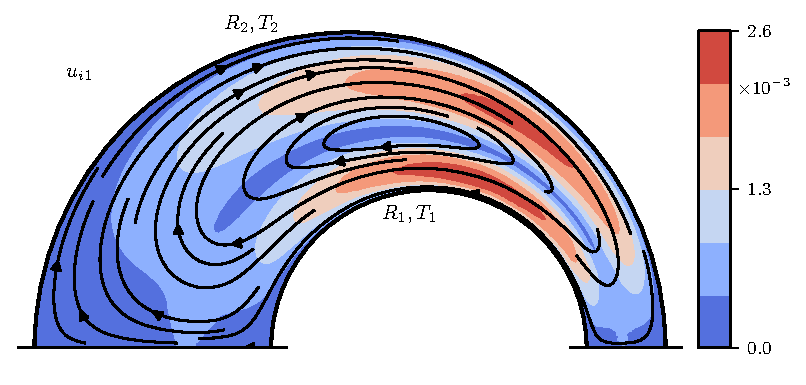
\includegraphics{Fig7}
	\caption{The velocity field \(u_{i1}\) between two noncoaxial cylinders:
		curves with arrows indicate the direction, contour lines show the magnitude.}
	\label{fig:cylinders}
\end{figure}

\begin{figure}
	\centering
	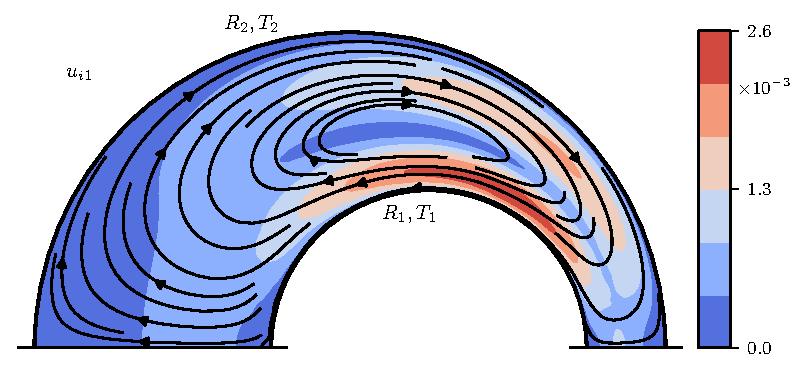
\includegraphics{Fig8}
	\caption{The velocity field \(u_{i1}\) between two nonconcentric spheres:
		curves with arrows indicate the direction, contour lines show the magnitude.}
	\label{fig:spheres}
\end{figure}

Now, consider the case, where there is no temperature gradient on the surface of the surrounding bodies at rest.
As stated above, even under such boundary conditions, convection flow can emerge
due to nonparallelism of the isothermal surfaces~\eqref{eq:equilibrium}.
This phenomenon is called the \emph{nonlinear thermal-stress flow}
and is described first in~\cite{Kogan1971}.
The nonlinear origin of this effect in the first order of the Knudsen number is relevant,
because a linear thermal-stress flow appears only in the following order of smallness \(O(k^2)\).
This type of convection has a important feature. It can occur in the state of weightlessness
whereas a gas convection in classical sense can be driven only by a finite gravity field.

Consider two cylinders of radius \(R_1 = 1\) and \(R_2 = r\)
with temperatures \(T_1 = 1\) and \(T_2 = \alpha\), respectively.
The cylinder axes are parallel; the distance between them is equal to \(d\).

Fig.~\ref{fig:cylinders} presents the results of numerical simulation for
\[ r = 2, \quad d = 1/2, \quad \alpha = 2. \]
The velocity field \(u_{i1}\) for this problem is much weaker than in the previous example,
so it has too small influence on the temperature distribution that we skip to demonstrate.

Gas between nonconcentric spheres is simulated in the same geometry,
as is between noncoaxial cylinders~\ref{fig:spheres}.

\subsection{Gas between two elliptical cylinders}

\begin{figure}
	\centering
	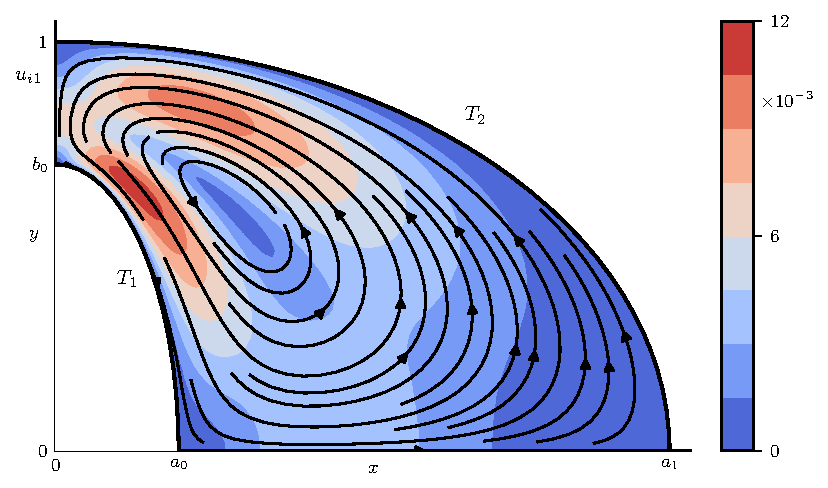
\includegraphics{Fig9}
	\caption{The velocity field \(u_{i1}\) between coaxial elliptical cylinders:
		curves with arrows indicate the direction, contour lines show the magnitude.}
	\label{fig:elliptic}
\end{figure}

In the last example, the gas is placed between two coaxial elliptical cylinders
in such a way that the major axes of the ellipses in a cross section are perpendicular.
Let the semi-minor axis of the outer cylinder be the characteristic length, while the semi-major one is \(a_1\).
The semi-axes of the inner ellipse are \(b_0\) and \(a_0\) in length, respectively.
The temperatures are equal to \(T_1 = 1\), \(T_2 = \alpha\) again.

In Fig.~\ref{fig:elliptic} the velocity field is shown for
\[ a_1 = 1.5, \quad a_0 = 0.3, \quad b_0 = 0.7, \quad \alpha = 2. \]
Numerical simulation of a rarefied gas using the DSMC method in the same geometry
for a wide range of Knudsen numbers \(0.1\le\Kn\le5\) can be found in~\cite{SoneCoaxial}.

\begin{figure}[ht]
	\centering
	\begin{minipage}{.48\textwidth}
		\centering
		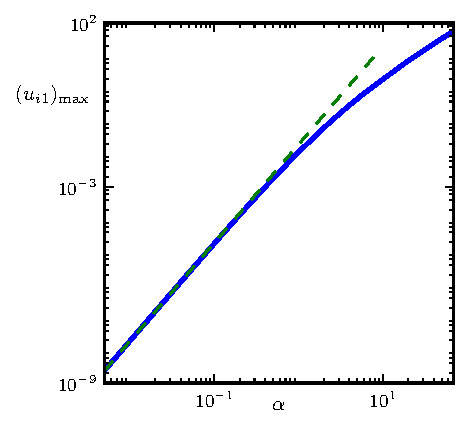
\includegraphics{Fig10}
		\caption{The maximum magnitude of \(u_{i1}\) versus the temperature ratio of the cylinders \(\alpha\).
			The dashed line corresponds the cubic relation.}
		\label{fig:maxU}
	\end{minipage}
	\quad
	\begin{minipage}{.48\textwidth}
		\centering
		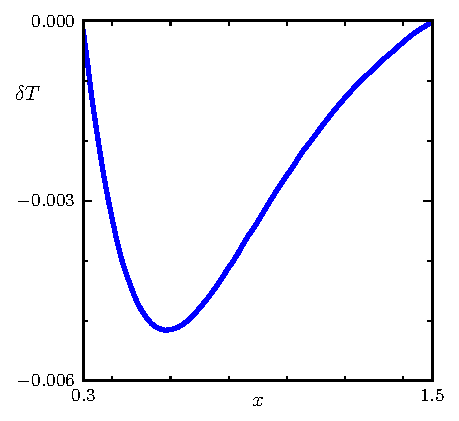
\includegraphics{Fig11}
		\caption{Difference between temperature distributions \(\delta T\) of the heat-conduction equation
			and the asymptotic theory along the \(x\) for \(\alpha = 5\).}
		\label{fig:deltaT}
	\end{minipage}
\end{figure}

Calculation of presented problems on the modern personal computer (3.40GHz CPU)
takes about several minutes for the most detailed spacial grids.
This fact provides a great performance for parametric studies as well. As an example,
the maximum magnitude of \(u_{i1}\) as a function of \(\alpha\) is shown in Fig.~\ref{fig:maxU}.
For small \(\alpha\),
\begin{equation}
	\mathrm{max}(u_{i1}) \propto \alpha^3, \quad \alpha\to0.
\end{equation}

Finally, Fig.~\ref{fig:deltaT} illustrates the discrepancy between the temperature fields
obtained from the asymptotic theory and the heat-conduction equation
\( \delta T = T_\mathrm{asym} - T_\mathrm{heat} \)
along the major axis of the outer cylinder.

\section{Conclusion}

%%% What it has been shown and achieved?
In the present paper, OpenFOAM\textregistered{}, a free and open-source CFD platform,
widely used and rapidly extending, is upgraded to deal with
slightly rarefied gas flows driven by significant temperature variations.
A reliable and rapid solver has been introduced on the basis of the appropriate
equations and boundary conditions, derived from the asymptotic analysis of the Boltzmann equation.
The program code has been validated by means of some benchmark simulations,
presented as illustrations. Typical problems of the first order of Knudsen number
have been considered: thermal creep flow and nonlinear thermal-stress flow.

%%% The meaning for the field
OpenFOAM\textregistered{}, together with the newly implemented numerical algorithm,
is an robust tool for numerical analysis of slightly rarefied gas problems
on the kinetic basis. The principal advantage of the developed code is that
it is easily extensible as an open-source software.

%%% Possible applications and extensions
Hard-sphere gas and diffuse reflection are considered in this paper,
but various molecular models and boundary conditions can be used as well.
In addition, appropriate equations for gas mixtures can be also naturally implemented.

\bibliographystyle{spphys} % spbasic, spmpsci, spphys
\bibliography{springer}

\end{document}


